% !TeX root = ../hw4.tex
\section{Reproducing the Gray-Scott Model Results}

\subsection{Statement}
Reproduce the Gray-Scott patterns $\alpha$, $\lambda$, $\mu$, and $\theta$ shown in \autoref{prob5:fig:patterns}.

\begin{figure}[H]
    \centering
    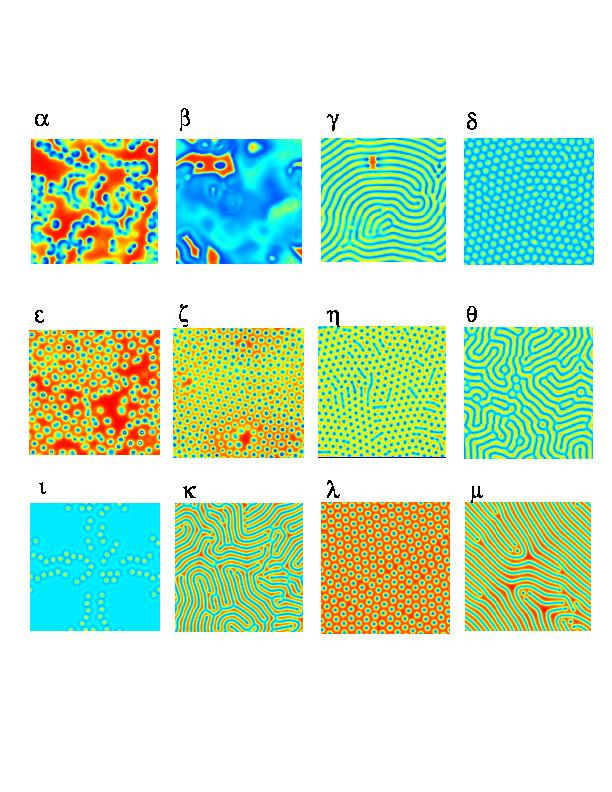
\includegraphics[width=0.6\textwidth]{figures/reactions/patterns.jpg}
    \caption{The labeled Gray-Scott patterns}\label{prob5:fig:patterns}
\end{figure}

\subsection{Method}

The Gray-Scott Model models reaction diffusion of two chemicals $U$ and $V$ in an unstirred planar chemical reactor.
Further, we assume the reaction $U \to V$ is autocatalyzed by the presence of $V$.
More specifically, the Gray-Scott model assumes the cubic autocatalysis
\begin{equation}
    U + 2V \to 3V
\end{equation}
with reaction rate $kuv^2$.
This reaction can be modeled according to the following system of differential equations.\footnote{I'm smashing my giant red ``I Believe'' button on this one. My chemistry is a little rusty, and PDEs give me heart palpitations.}
\begin{equation}
    \begin{cases}
        \displaystyle{\frac{\partial u}{\partial t} = r_u \Delta u - uv^2 + f(1 - u)} \\[10pt]
        \displaystyle{\frac{\partial v}{\partial t} = r_v \Delta v + uv^2 - (f + k)v}
    \end{cases}\label{prob5:eqn:gray-scott}
\end{equation}
where $u$ and $v$ are the concentrations, and $r_u$ and $r_v$ are the diffusion rates, of $U$ and $V$ respectively.
The chemical $U$ is added to the reactor at the feed rate $f$ which is scaled by the concentration of $U$.
Simultaneously, $U$ and $V$ are drained from the reactor at the kill rate $k$, which is scaled by $f$ and the concentration of $V$.

Recall that the Laplacian operator $\displaystyle\Delta f(x, y, t) = \nabla^2 f(x, y, t) = \frac{\partial^2 f}{\partial x^2} + \frac{\partial^2 f}{\partial y^2}$ can be discretized as
\begin{align}
    \Delta f(x, y, t) \approx \frac{f(x - h, y, t) + f(x + h, y, t) + f(x, y - h, t) + f(x, y + h, t) - 4f(x, y)}{h^2}\label{prob5:eqn:discrete-laplacian-operator}
\end{align}
for fixed step size $h$, uniform in both spatial dimensions --- allowing us to collect more of the terms together.
In this problem, we have $\Delta x = \Delta y = \Delta t = h = 1$.

However, note that the numerical computation of $\Delta f$ over a large spatial domain is computationally intensive, despite being relatively simple.
Therefore, we desire a a method where the Laplacian can be applied to $f$ over each element of the spatial domain at once.

Let $\mathbf U$ be a square $n \times n$ matrix of concentrations.
We then unravel $\mathbf U$ into a column vector $\vec u$ and left-multiply by an $n^2 \times n^2$ matrix $\mathbf L$ to numerically compute the discrete Laplacian over the entire spatial domain.

That is, the discretized version of \autoref{prob5:eqn:gray-scott} becomes
\begin{eqnarray}
    \begin{cases}
        \vec u_{t + 1} & = \vec u_t + r_u \mathbf L \cdot \vec u_t - \vec u_t \cdot \vec {v_t}^2 + f(1 - \vec u_t) \\
        \vec v_{t + 1} & = \vec v_t + r_v \mathbf L \cdot \vec v_t + \vec u_t \cdot \vec {v_t}^2 - (f + k)\vec v_t
    \end{cases}\label{prob5:eqn:discretized-gray-scott}
\end{eqnarray}
where the vector product $\vec u_t \cdot \vec {v_t}^2$ is computed component-wise.

Then the $n ^2 \times n^2$ matrix $\mathbf L$ is the block diagonal matrix
\begin{equation}
    \mathbf L = \begin{bmatrix}
        L_n    & I_n    & 0_n    & \cdots & 0_n    & I_n    \\
        I_n    & L_n    & I_n    & 0_n    & \cdots & 0_n    \\
        0_n    & I_n    & L_n    & I_n    & \ddots & \vdots \\
        \vdots & \ddots & \ddots & \ddots & \ddots & 0_n    \\
        0_n    & \cdots & 0_n    & I_n    & L_n    & I_n    \\
        I_n    & 0_n    & \cdots & 0_n    & I_n    & L_n
    \end{bmatrix}\label{prob5:eqn:laplacian}
\end{equation}
where the $0_n$ blocks are the $n \times n$ zero matrix, and the $I_n$ blocks are the $n \times n$ identity matrix.
The $L_n$ blocks are the $n \times n$ diagonal matrix
\begin{equation}
    L_n = \begin{bmatrix}
        -4     & 1      & 0      & \cdots & 0      & 1      \\
        1      & -4     & 1      & 0      & \cdots & 0      \\
        0      & 1      & -4     & 1      & \ddots & \vdots \\
        \vdots & \ddots & \ddots & \ddots & \ddots & 0      \\
        0      & \cdots & 0      & 1      & -4     & 1      \\
        1      & 0      & \cdots & 0      & 1      & -4
    \end{bmatrix}\label{prob5:eqn:laplacian-L-block}
\end{equation}

Now, $\mathbf L$ is appropriate for periodic boundary conditions.
If homogeneous Dirichlet boundary conditions are desired, we use the matrix
\begin{equation}
    \mathbf L_d = \begin{bmatrix}
        L_n              & I_n    & 0_n    & \cdots & 0_n    & \color{red}{0_n} \\
        I_n              & L_n    & I_n    & 0_n    & \cdots & 0_n              \\
        0_n              & I_n    & L_n    & I_n    & \ddots & \vdots           \\
        \vdots           & \ddots & \ddots & \ddots & \ddots & 0_n              \\
        0_n              & \cdots & 0_n    & I_n    & L_n    & I_n              \\
        \color{red}{0_n} & 0_n    & \cdots & 0_n    & I_n    & L_n
    \end{bmatrix}
\end{equation}
and the modified $L_n$ block
\begin{equation}
    L_n = \begin{bmatrix}
        -4             & 1      & 0      & \cdots & 0      & \color{red}{0} \\
        1              & -4     & 1      & 0      & \cdots & 0              \\
        0              & 1      & -4     & 1      & \ddots & \vdots         \\
        \vdots         & \ddots & \ddots & \ddots & \ddots & 0              \\
        0              & \cdots & 0      & 1      & -4     & 1              \\
        \color{red}{0} & 0      & \cdots & 0      & 1      & -4
    \end{bmatrix}
\end{equation}
If homogeneous Neumann boundary conditions are desired, further modifications must be made to the main diagonal of $\mathbf L_d$ to maintain 0-sum rows.\footnote{
    Online material on the discretized Laplacian is lacking in general, and much more so related to periodic boundary conditions.
    I found exactly one source that discussed the discretized Laplacian with periodic boundary conditions in more than one sentence.

    A PDF of \textit{Computational Methods for Inverse Problems} may be found on \href{http://booksdescr.org/item/index.php?md5=6DF2AA596DDBE34BCF9354A5626B75DA}{Library Genesis}.
    The relevant pages are 74--75.
}

\subsection{Implementation}
\subsection{Results}
The $f$ and $k$ parameters largely decide the pattern displayed at the end of a large number of iterations.
The mappings for the patterns shown in \autoref{prob5:fig:patterns} are shown in \autoref{prob5:fig:pattern-mappings}.
\begin{figure}[H]
    \centering
    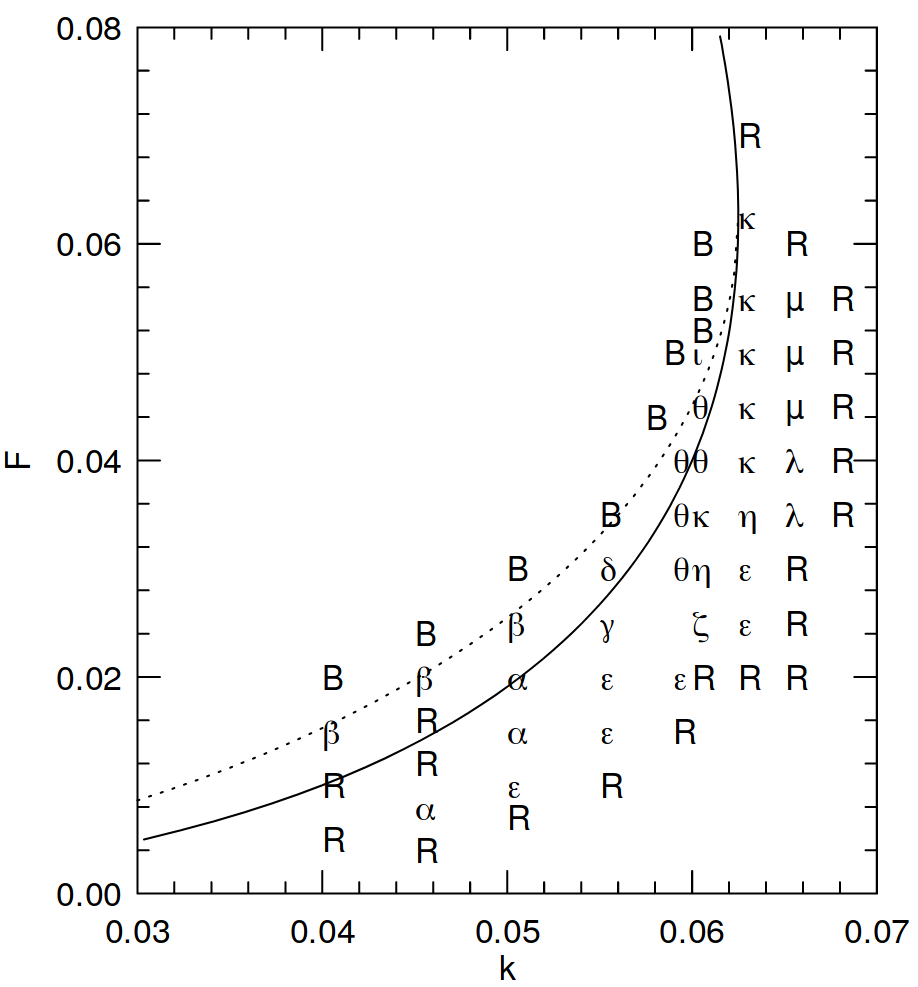
\includegraphics[width=0.6\textwidth]{figures/reactions/pattern-mappings.png}
    \caption{The parameter mappings to the patterns shown in \autoref{prob5:fig:patterns}}\label{prob5:fig:pattern-mappings}
\end{figure}
\subsection{Conclusion}
